\begin{uebsp}
\begin{Exercise}[label=ex:1.5]
Die symmetrische Differenz von zwei Mengen (''exklusives Oder'') ist

\[A\Delta B=(A\\B)\cup (B\\A)\]

Bestimmen Sie Ausdrücke für $\mathbb{P}(A\Delta B)$ und $\mathbb{P}(A\Delta B\Delta C)$\\

(Zusatzaufgabe: Raten Sie, wie die Formel für $n$-Mengen aussieht)
\end{Exercise}
\begin{Answer}
    \begin{enumerate}[i)]
        \item Ausdruck für $A\Delta B$:
            \begin{multicols}{2}
                \[\mathbb{P}(A\Delta B)=\mathbb{P}(A)-\mathbb{P}(A\cap B)+\mathbb{P}(B)-\mathbb{P}(A\cap B)\]
                \[\mathbb{P}(A\Delta B)=\mathbb{P}(A)+\mathbb{P}(B)-2\mathbb{P}(A\cap B)\]
                \columnbreak

                \begin{tikzpicture}
                \input{examples/round1/2circ}
                \end{tikzpicture}
            \end{multicols}
        \item Ausdruck für $A\Delta B\Delta C$:
            \begin{multicols}{2}
            \begin{align*}  &\mathbb{P}(A\Delta B\Delta C)=\\
                            &=\mathbb{P}(A)-\mathbb{P}(A\cap B)-\mathbb{P}(A\cap C)\\
                            &+\mathbb{P}(B)-\mathbb{P}(A\cap B)-\mathbb{P}(B\cap C)\\
                            &+\mathbb{P}(C)-\mathbb{P}(A\cap C)-\mathbb{P}(B\cap C)\\
                            &+4\mathbb{P}(A\cap B\cap C)\end{align*}
            \begin{align*}&\mathbb{P}(A\Delta B\Delta C)=\\&=\mathbb{P}(A)+\mathbb{P}(B)+\mathbb{P}(C)-2\mathbb{P}(A\cap B)-2\mathbb{P}(A\cap C)-2\mathbb{P}(B\cap C)+4\mathbb{P}(A\cap B\cap C)\end{align*}
                \columnbreak

                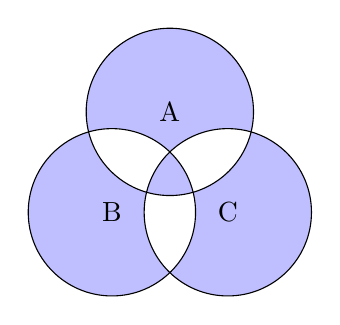
\begin{tikzpicture}[scale=0.85]
                    {
    \def\firstcircle{(90:1cm) circle (1.25cm)}
    \def\secondcircle{(210:1cm) circle (1.25cm)}
    \def\thirdcircle{(330:1cm) circle (1.25cm)}


    \fill[blue!25] \firstcircle;
    \fill[blue!25] \secondcircle;
    \fill[blue!25] \thirdcircle;

    \begin{scope}
        \clip \firstcircle;
        \fill[white] \secondcircle;
    \end{scope}
    \begin{scope}
        \clip \firstcircle;
        \fill[white] \thirdcircle;
    \end{scope}
    \begin{scope}
        \clip \secondcircle;
        \fill[white] \thirdcircle;
    \end{scope}

    \begin{scope}
        \clip \firstcircle;
        \clip \secondcircle;
        \fill[blue!25] \thirdcircle;
    \end{scope}

    \draw \firstcircle node {A};
    \draw \secondcircle node {B};
    \draw \thirdcircle node {C};
}

                \end{tikzpicture}
            \end{multicols}
            
            \textbf{Achtung:} da die Schnittmenge von $A\cap B\cap C$(also der Mittelpunkt) zur Symmetrischen Differenz dazugehört, folgt:
            $+4\mathbb{P}(A\cap B\cap C)$, da die Schnittmenge $3$-mal addiert wird, dann $6$-mal subtrahiert wird, muss sie folglich $4$-mal addiert werden. ($3x-6x+4x=1x$)
        \item Ausdruck für $n$-Mengen:
            \[\mathbb{P}(A_1\Delta A_2\Delta ...\Delta A_n)=\sum_{k=1}^n(-1)^{k-1}\cdot 2^{k-1}\cdot S_k\]
            \[\text{wobei } S_k=\sum_{1\leq i_1\leq i_2\leq ...\leq i_k \leq n}\mathbb{P}(A_{i_1}\cap A_{i_2}\cap ...\cap A_{i_k})\]
    \end{enumerate}
\end{Answer}
\end{uebsp}
